\documentclass[11pt]{article}
\usepackage[textwidth=18.0cm, textheight=23.0cm, top=2.0cm]{geometry}
\usepackage{pst-all}
\usepackage{amssymb}
\usepackage{tikz}
\usepackage{underscore}\begin{document}
\pagestyle{empty}


ClassName: \underline{\textbf{Class_08.2bp-1}}
\par
BinSize: \underline{\textbf{100 × 100}}
\par
ReduceSize: \underline{\textbf{100 × 100}}
\par
TypeNum: \underline{\textbf{20}}
\par
Num: \underline{\textbf{20}}
\par
OutS: \underline{\textbf{70000}}
\par
InS: \underline{\textbf{46400}}
\par
Rate: \underline{\textbf{0.663}}
\par
UB: \underline{\textbf{7}}
\par
LB0: \underline{\textbf{7}}
\par
LB: \underline{\textbf{7}}
\par
LBWithCut: \underline{\textbf{7}}
\par
NodeCut: \underline{\textbf{0}}
\par
ExtendedNodeCnt: \underline{\textbf{1}}
\par
GenNodeCnt: \underline{\textbf{1}}
\par
PrimalNode: \underline{\textbf{0}}
\par
ColumnCount: \underline{\textbf{7}}
\par
TotalCutCount: \underline{\textbf{0}}
\par
RootCutCount: \underline{\textbf{0}}
\par
LPSolverCnt: \underline{\textbf{1}}
\par
PricingSolverCnt: \underline{\textbf{0}}
\par
BranchAndBoundNum: \underline{\textbf{1}}
\par
isOpt: \underline{\textbf{true}}
\par
TimeOnInitSolution: \underline{\textbf{0.010 s}}
\par
TimeOnPrimal: \underline{\textbf{0.000 s}}
\par
TimeOnPricing: \underline{\textbf{0.000 s}}
\par
TimeOnRmp: \underline{\textbf{0.063 s}}
\par
TotalTime: \underline{\textbf{0.120 s}}
\par
\newpage


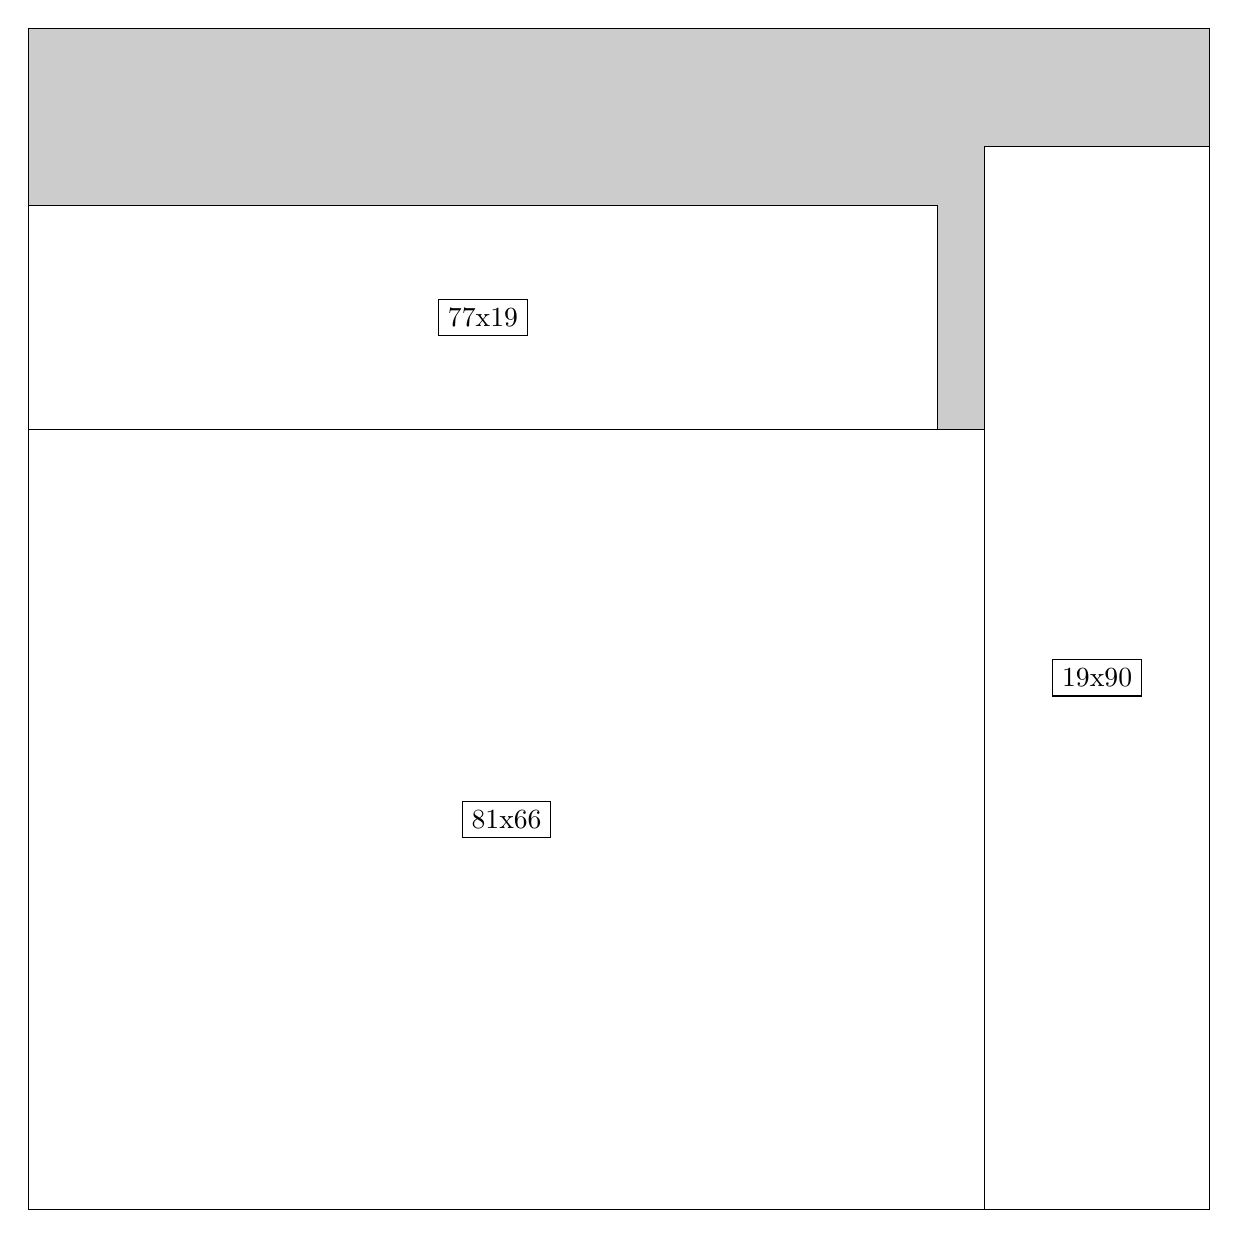
\begin{tikzpicture}[shorten >=1pt,scale=1.0,every node/.style={scale=1.0},->]
\tikzstyle{vertex}=[circle,fill=black!25,minimum size=14pt,inner sep=0pt]
\filldraw[fill=gray!40!white, draw=black] (0,0) rectangle (15.0,15.0);
\foreach \name/\x/\y/\w/\h in {81x66/0.0/0.0/12.15/9.9,19x90/12.15/0.0/2.85/13.5,77x19/0.0/9.9/11.549999999999999/2.85}
\filldraw[fill=white!40!white, draw=black] (\x,\y) rectangle node[draw] (\name) {\name} ++(\w,\h);
\end{tikzpicture}


w =81 , h =66 , x =0 , y =0 , v =5346
\par
w =19 , h =90 , x =81 , y =0 , v =1710
\par
w =77 , h =19 , x =0 , y =66 , v =1463
\par
\newpage


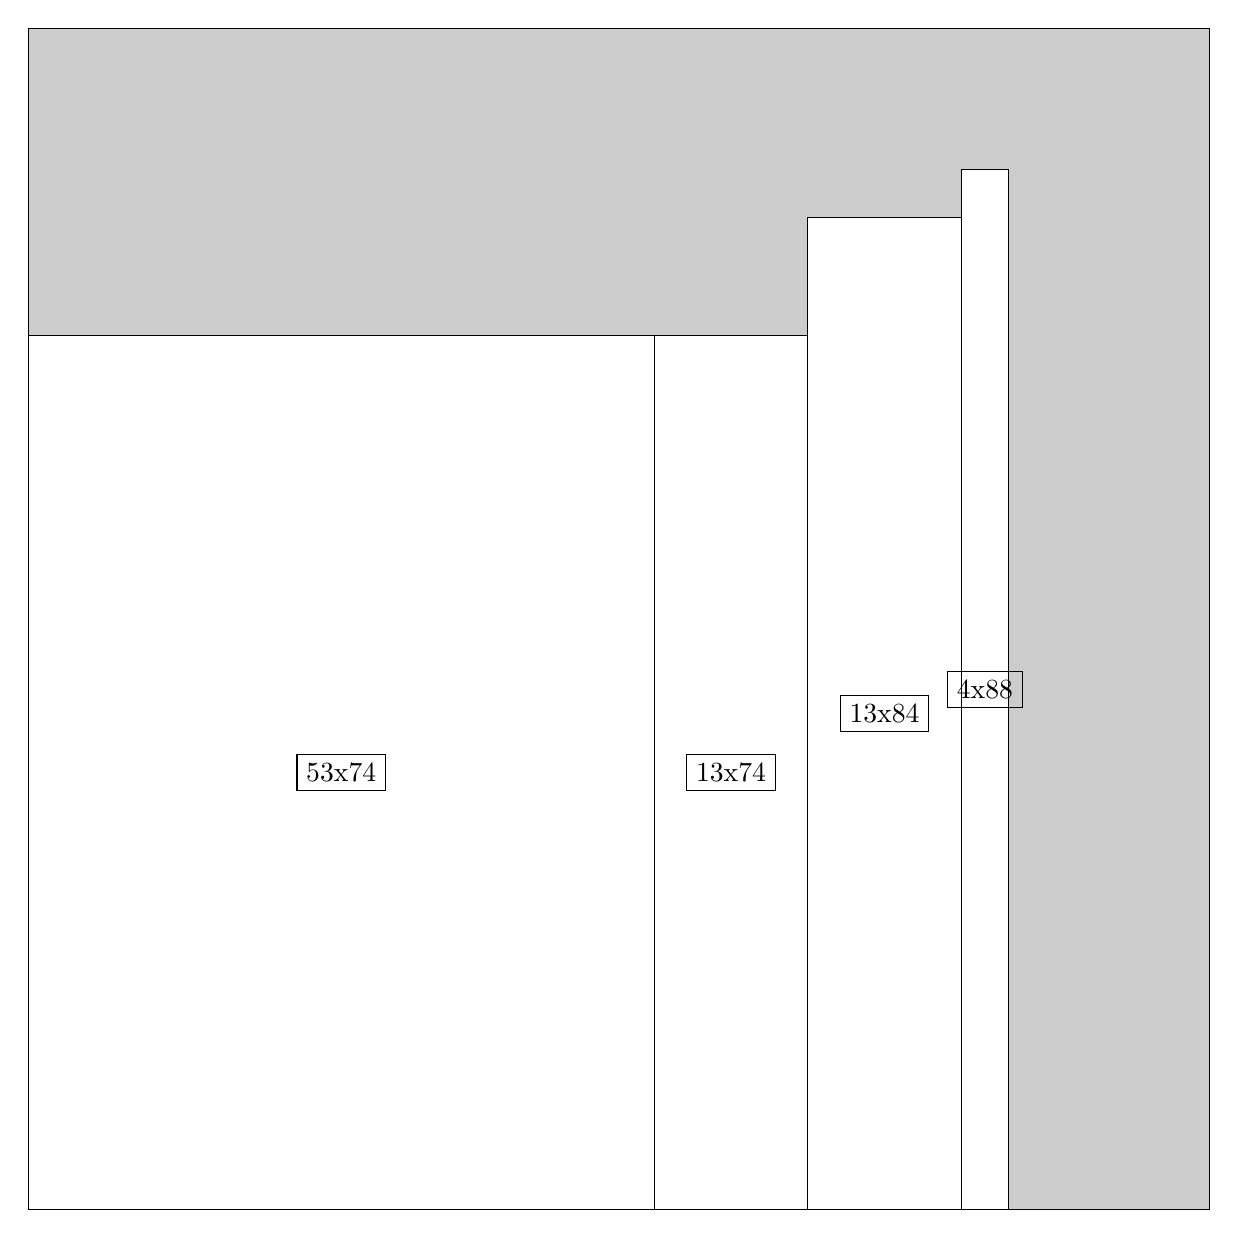
\begin{tikzpicture}[shorten >=1pt,scale=1.0,every node/.style={scale=1.0},->]
\tikzstyle{vertex}=[circle,fill=black!25,minimum size=14pt,inner sep=0pt]
\filldraw[fill=gray!40!white, draw=black] (0,0) rectangle (15.0,15.0);
\foreach \name/\x/\y/\w/\h in {53x74/0.0/0.0/7.949999999999999/11.1,13x84/9.9/0.0/1.95/12.6,13x74/7.949999999999999/0.0/1.95/11.1,4x88/11.85/0.0/0.6/13.2}
\filldraw[fill=white!40!white, draw=black] (\x,\y) rectangle node[draw] (\name) {\name} ++(\w,\h);
\end{tikzpicture}


w =53 , h =74 , x =0 , y =0 , v =3922
\par
w =13 , h =84 , x =66 , y =0 , v =1092
\par
w =13 , h =74 , x =53 , y =0 , v =962
\par
w =4 , h =88 , x =79 , y =0 , v =352
\par
\newpage


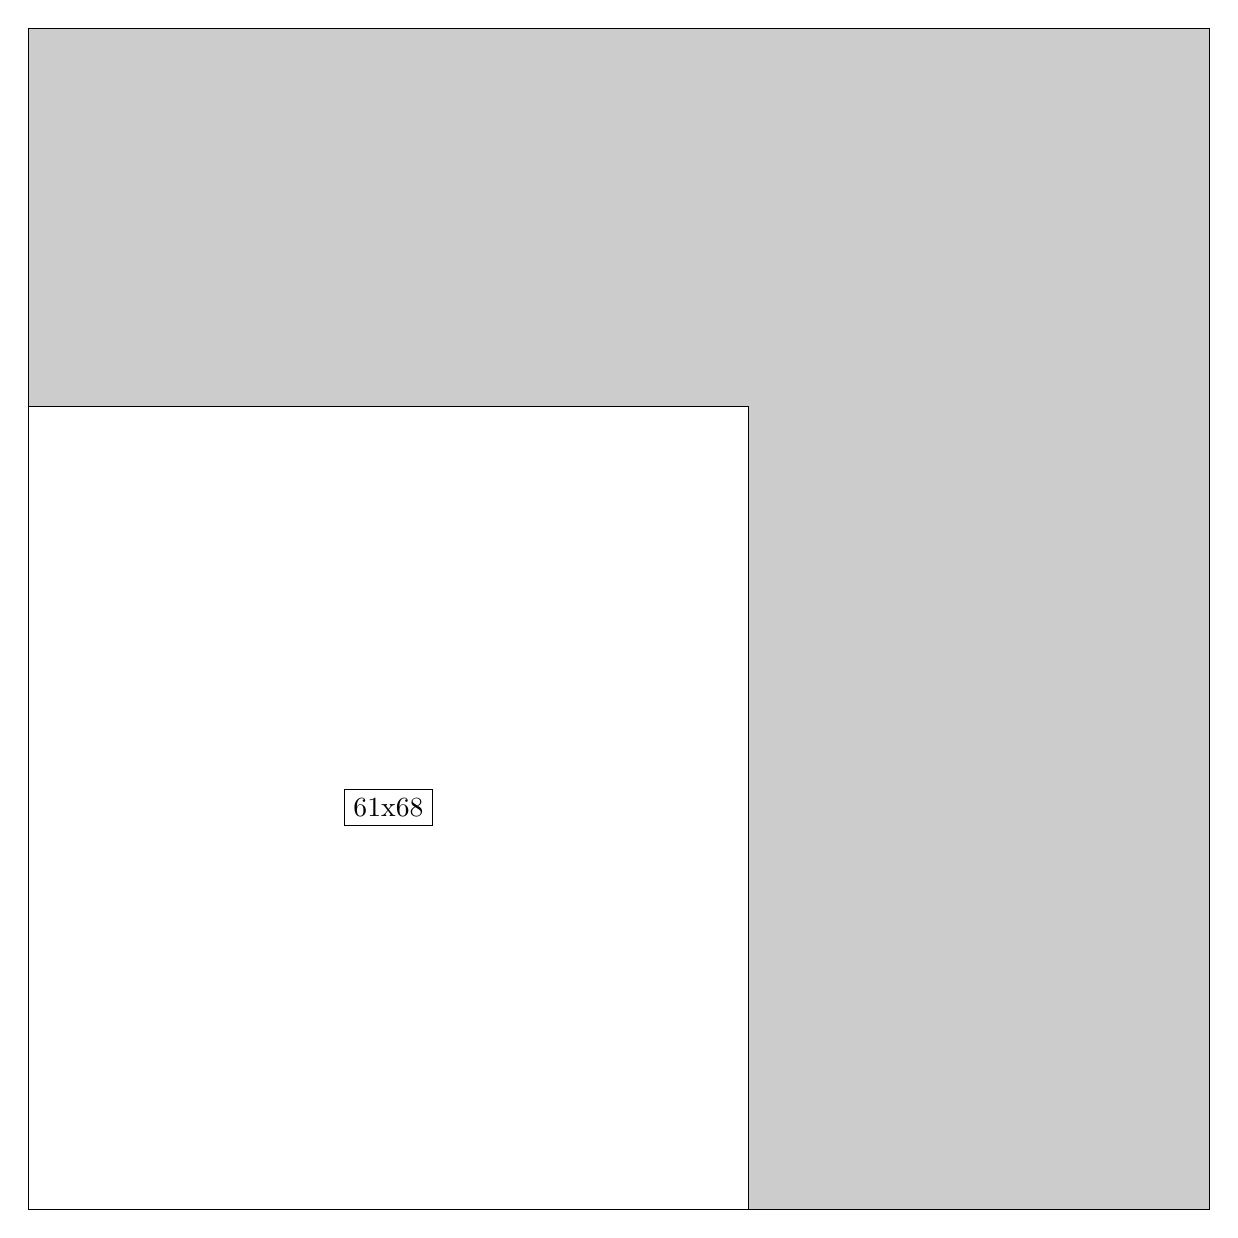
\begin{tikzpicture}[shorten >=1pt,scale=1.0,every node/.style={scale=1.0},->]
\tikzstyle{vertex}=[circle,fill=black!25,minimum size=14pt,inner sep=0pt]
\filldraw[fill=gray!40!white, draw=black] (0,0) rectangle (15.0,15.0);
\foreach \name/\x/\y/\w/\h in {61x68/0.0/0.0/9.15/10.2}
\filldraw[fill=white!40!white, draw=black] (\x,\y) rectangle node[draw] (\name) {\name} ++(\w,\h);
\end{tikzpicture}


w =61 , h =68 , x =0 , y =0 , v =4148
\par
\newpage


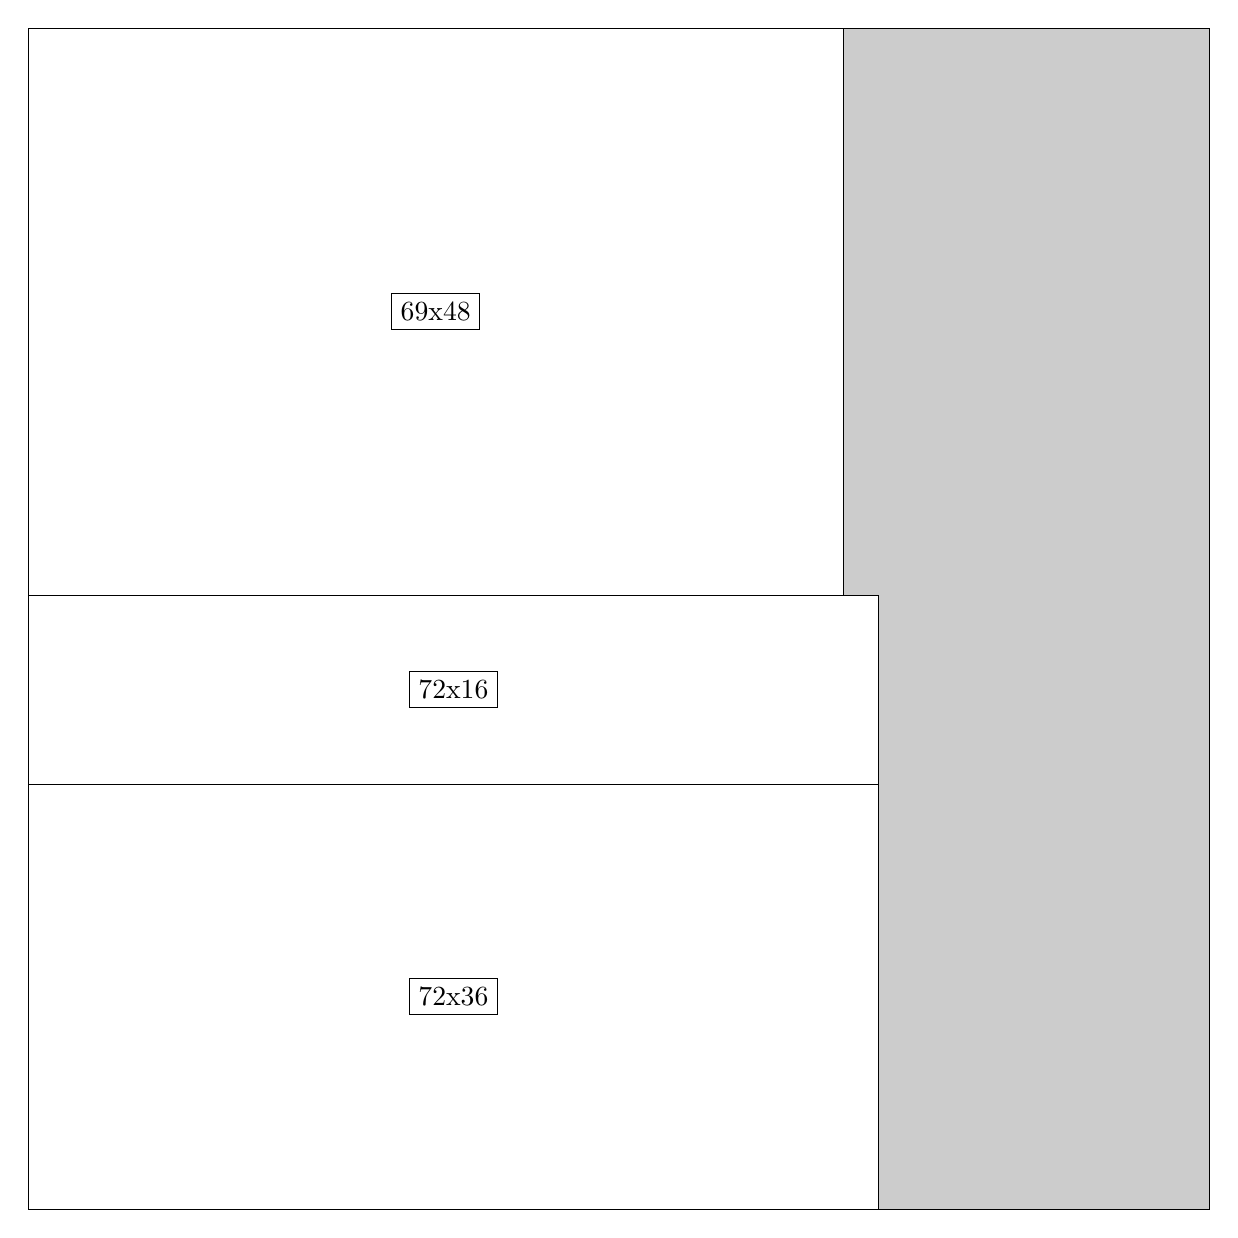
\begin{tikzpicture}[shorten >=1pt,scale=1.0,every node/.style={scale=1.0},->]
\tikzstyle{vertex}=[circle,fill=black!25,minimum size=14pt,inner sep=0pt]
\filldraw[fill=gray!40!white, draw=black] (0,0) rectangle (15.0,15.0);
\foreach \name/\x/\y/\w/\h in {72x36/0.0/0.0/10.799999999999999/5.3999999999999995,69x48/0.0/7.8/10.35/7.199999999999999,72x16/0.0/5.3999999999999995/10.799999999999999/2.4}
\filldraw[fill=white!40!white, draw=black] (\x,\y) rectangle node[draw] (\name) {\name} ++(\w,\h);
\end{tikzpicture}


w =72 , h =36 , x =0 , y =0 , v =2592
\par
w =69 , h =48 , x =0 , y =52 , v =3312
\par
w =72 , h =16 , x =0 , y =36 , v =1152
\par
\newpage


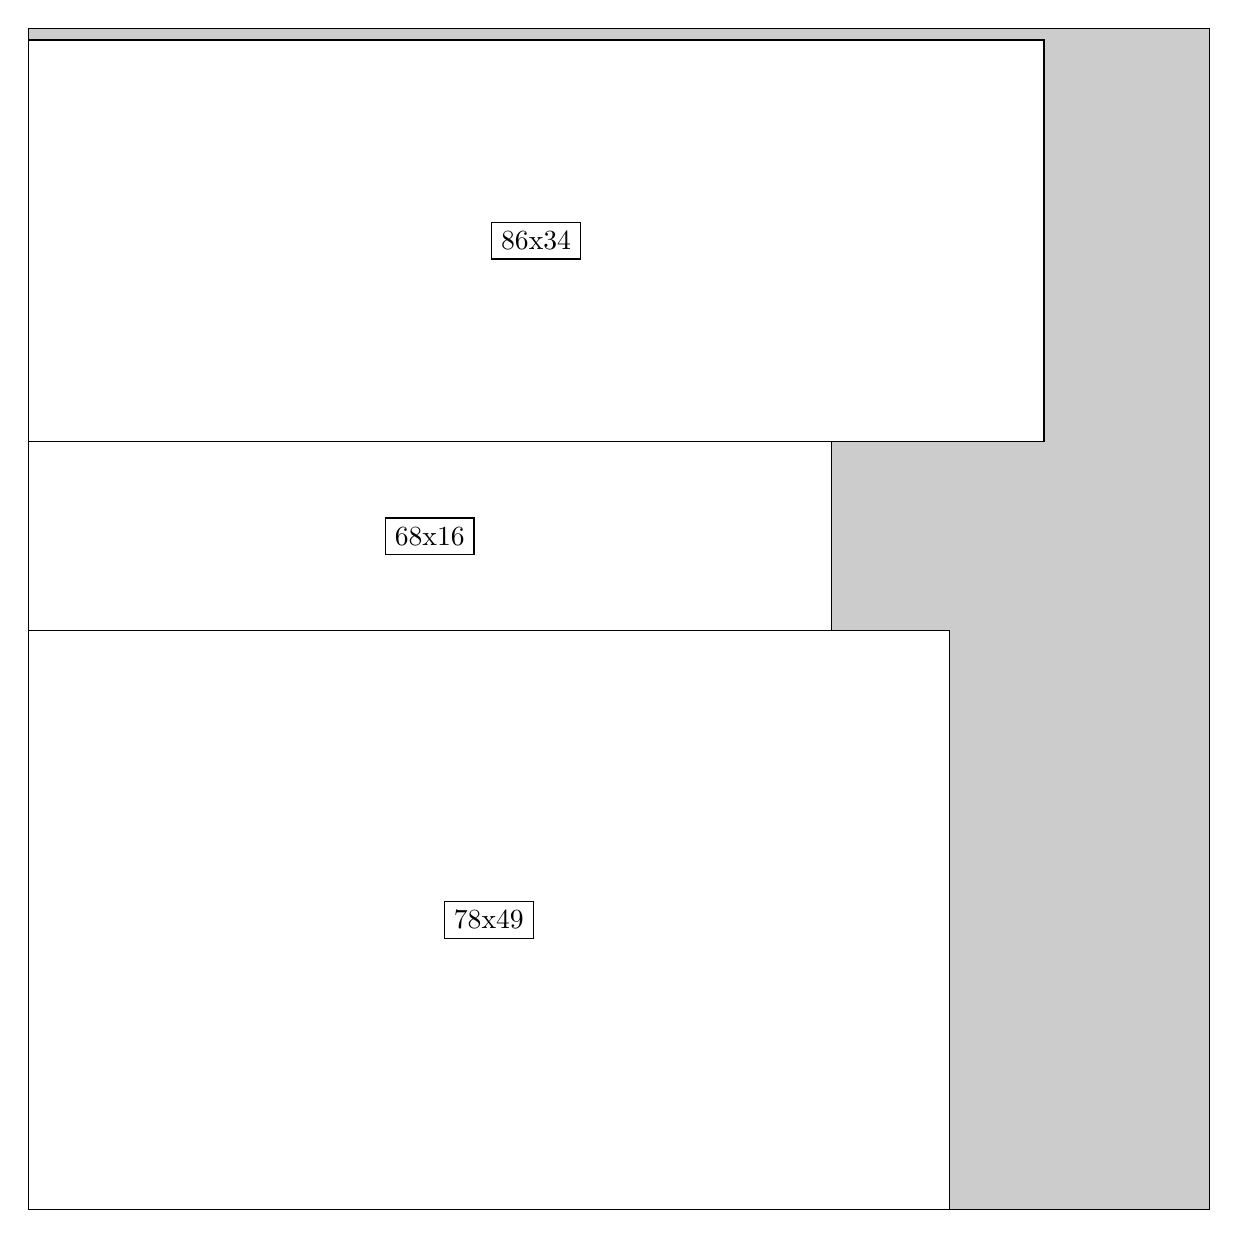
\begin{tikzpicture}[shorten >=1pt,scale=1.0,every node/.style={scale=1.0},->]
\tikzstyle{vertex}=[circle,fill=black!25,minimum size=14pt,inner sep=0pt]
\filldraw[fill=gray!40!white, draw=black] (0,0) rectangle (15.0,15.0);
\foreach \name/\x/\y/\w/\h in {78x49/0.0/0.0/11.7/7.35,86x34/0.0/9.75/12.9/5.1,68x16/0.0/7.35/10.2/2.4}
\filldraw[fill=white!40!white, draw=black] (\x,\y) rectangle node[draw] (\name) {\name} ++(\w,\h);
\end{tikzpicture}


w =78 , h =49 , x =0 , y =0 , v =3822
\par
w =86 , h =34 , x =0 , y =65 , v =2924
\par
w =68 , h =16 , x =0 , y =49 , v =1088
\par
\newpage


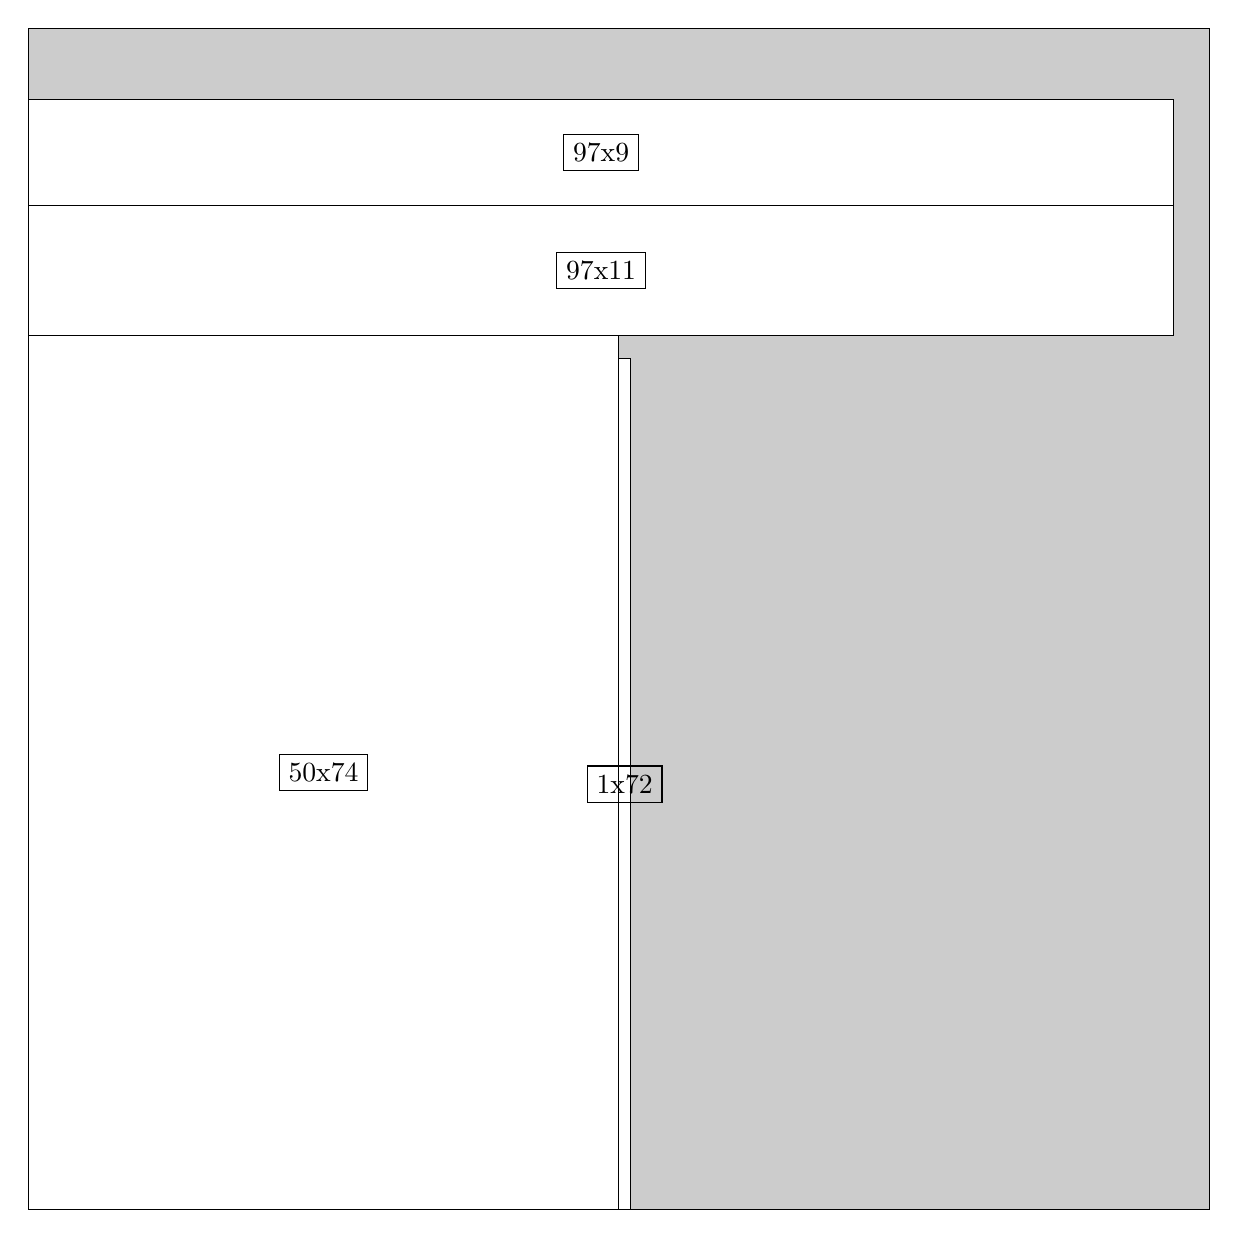
\begin{tikzpicture}[shorten >=1pt,scale=1.0,every node/.style={scale=1.0},->]
\tikzstyle{vertex}=[circle,fill=black!25,minimum size=14pt,inner sep=0pt]
\filldraw[fill=gray!40!white, draw=black] (0,0) rectangle (15.0,15.0);
\foreach \name/\x/\y/\w/\h in {50x74/0.0/0.0/7.5/11.1,97x11/0.0/11.1/14.549999999999999/1.65,97x9/0.0/12.75/14.549999999999999/1.3499999999999999,1x72/7.5/0.0/0.15/10.799999999999999}
\filldraw[fill=white!40!white, draw=black] (\x,\y) rectangle node[draw] (\name) {\name} ++(\w,\h);
\end{tikzpicture}


w =50 , h =74 , x =0 , y =0 , v =3700
\par
w =97 , h =11 , x =0 , y =74 , v =1067
\par
w =97 , h =9 , x =0 , y =85 , v =873
\par
w =1 , h =72 , x =50 , y =0 , v =72
\par
\newpage


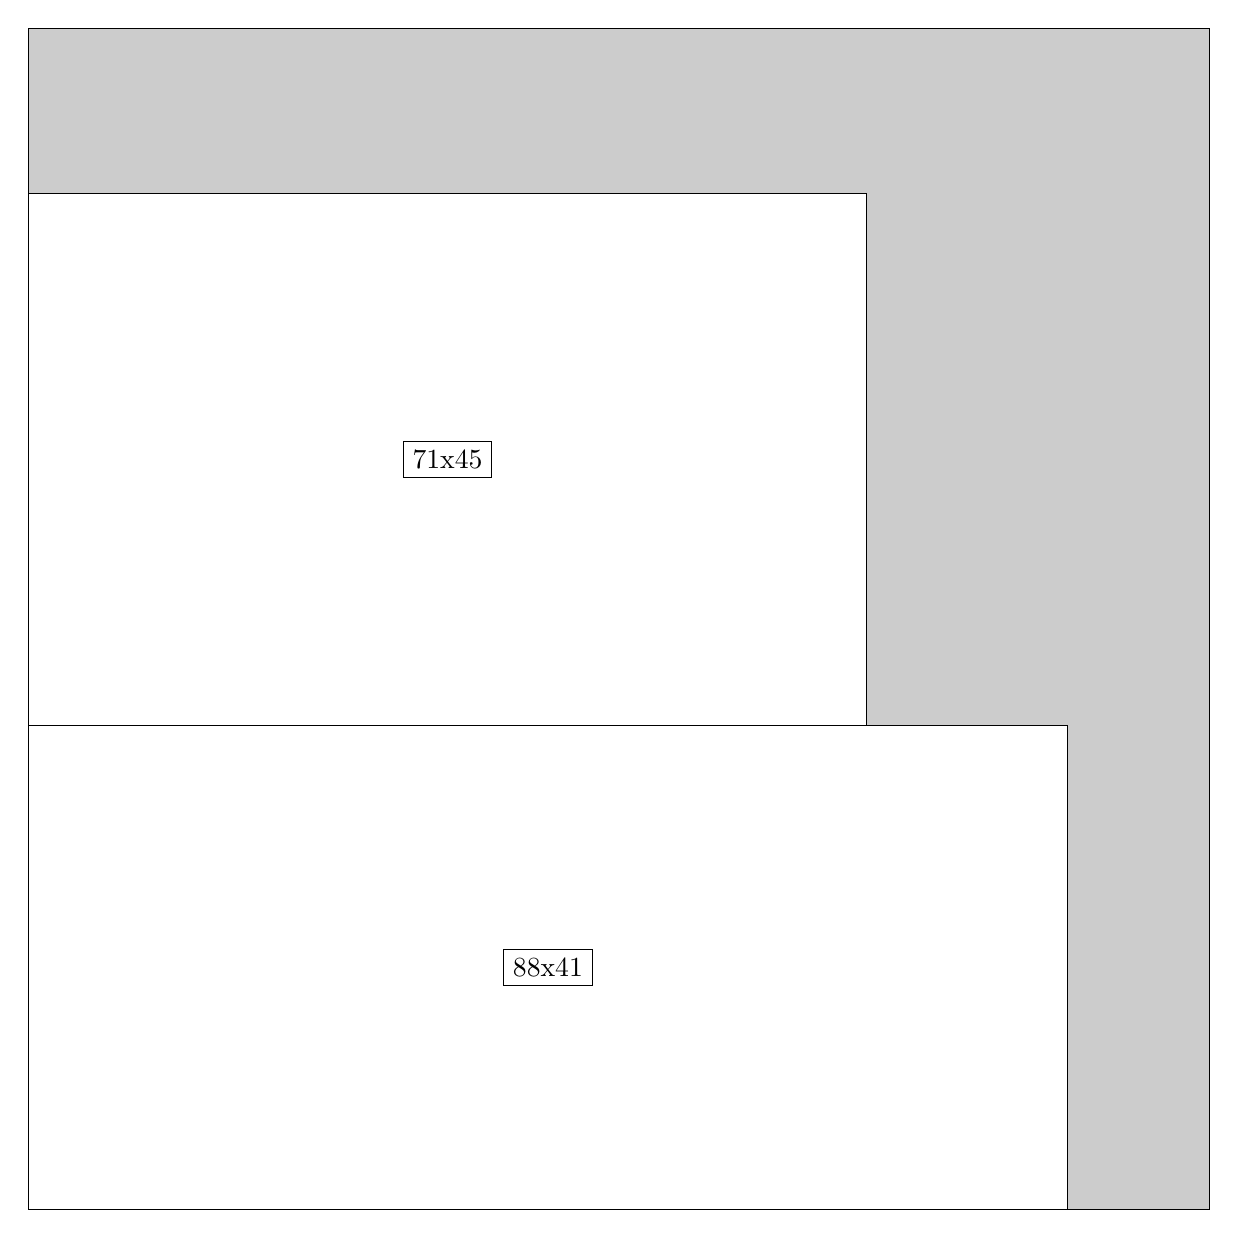
\begin{tikzpicture}[shorten >=1pt,scale=1.0,every node/.style={scale=1.0},->]
\tikzstyle{vertex}=[circle,fill=black!25,minimum size=14pt,inner sep=0pt]
\filldraw[fill=gray!40!white, draw=black] (0,0) rectangle (15.0,15.0);
\foreach \name/\x/\y/\w/\h in {88x41/0.0/0.0/13.2/6.1499999999999995,71x45/0.0/6.1499999999999995/10.65/6.75}
\filldraw[fill=white!40!white, draw=black] (\x,\y) rectangle node[draw] (\name) {\name} ++(\w,\h);
\end{tikzpicture}


w =88 , h =41 , x =0 , y =0 , v =3608
\par
w =71 , h =45 , x =0 , y =41 , v =3195
\par
\newpage


\end{document}